\documentclass[11pt,a4paper,oneside]{report}

\usepackage{url, enumitem}
\usepackage{amsfonts, amsmath}
\usepackage{graphicx, color}
\usepackage{algorithm}
\usepackage[toc,page]{appendix}
\usepackage{lmodern}
\usepackage{amsmath}
\usepackage{natbib}

% Some useful macros.
\newcommand{\given}{\,|\,}
\newcommand{\R}{\mathbb{R}}
\newcommand{\E}{\mathbb{E}}
\newcommand{\var}{\text{var}}
\newcommand{\cov}{\text{cov}}

\usepackage{float}
\floatplacement{figure}{H} % force figures to be placed always at defined position!
\begin{document}

\title{CS 283: Initial Proposal}
\author{Nicolas Drizard \\
Leonhard Spiegelberg}
\date{10/23/15}

\maketitle

\newpage

\section*{Introduction}

Looking for an applied project, we decided to take part in a Kaggle competition: Right Whale Recognition! The objective of this competition is to build a program to recognize right whales in aerial photographies, given a training set with $500$ (North Atlantic) right whales. The dataset is constituted of $11,468$ aerial photographies with only one whale. Among these pictures, $4,545$ are already labeled with the ID of one of the $500$ whales. The main characteristics which help to differentiate one whale from another are the white callosities (roughened patches of skin) on their head.\\
\\

In this proposal, we first discuss some of the challenges of this problem and then present a potential roadmap to address this problem.


\section*{Challenges}

One of the main challenges with this problem relies in the feature engineering part. The images are raw pictures taken by a scientist with a normal camera and the whale is most of the time hard to recognize even with the naked eye. Different elements may perturb our work:
\begin{itemize}
	\item different lighting conditions need to addressed in the preprocessing step
	\item foam on the water has nearly the same color like the callosities we want to recognize. As foam takes nearly every shape, this will cause a lot of 'foam' features that will be incorrectly classified as callosities
	\item the orientation and position of the whale impacts visibility of the features, i.e. the whale can be half or more covered by water. Water refraction will change feature appearance.
\end{itemize}


\section*{Roadmap}
Given the lack of relevant information and the high level of noise in the pictures, we will use a progressive approach to solve this problem. \\
First, we will select a set of nice images (no distraction like foam, visible key features) to work on the feature engineering part to have a better understanding of the problem.\\
On these pictures, we will extract features. Two approaches may be considered. On the first hand, we extract a bag of features for each image (with SIFT for instance) and apply an algorithm to select the relevant features among them, i.e. the whale based one, and compare them (with a POOF approach for instance). On the other hand, we want to select directly the relevant features. Working on nice images makes this task easier as the noise is reduced. Then, we can apply the following classical feature extraction workflow:
\begin{enumerate}
	\item Preprocessing (i.e. normalizing luminance, converting channels, ...)
	\item Thresholding (extract pixels of interest, i.e. via a hysteresis approach)
   	\item Segmentation (Splitting the points into segments)
    	\item Feature estimation for each segment (i.e. half axes of ellipses, roundness measures, ...)
\end{enumerate}
Once we come up with relevant features, we run a classifier on the training set. We will focus on the feature engineering part so we will probably use a classical classifier as for instance SVM or regularized logistic regression. 


\section*{Implementation}
In order to classify a whale, we split the work in two parts. The first part consists of localizing the nose, its parts and extracting a feature vector from it for additional precision. The second part deals with the actual classification which shall be done using a part-based one-vs-one features (POOF) approach. 
\subsection*{Part I: Localizing the nose and parts of it[Leonhard]}
As mentioned in the introduction callosities and the shape or size of a head are main features to distinguish a whale from the others. In order to localize the nose and parts of it, an approach using histograms of gradients as described in \citep{dalal2005histograms}
%\url{http://lear.inrialpes.fr/people/triggs/pubs/Dalal-cvpr05.pdf}
shall be implemented. Histograms of Oriented Gradients (HOG) is a method proposed by Dalal \& Triggs in 2005 which has been used previously to detect humans in images. 
\\
\\
The idea behind HOG is to describe a local object's shape and appearance via a histogram of (binned) gradients. To detect objects (in our case the whole nose and its parts (i.e. callosities)) a sliding window is used to feed the gradient histograms into a classifier. A first design choice that has to be made is what kind of window should be used. In general, two reasonable choices are rectangular or circular windows. As in the given dataset whales are arbitrarily oriented for a first analysis a squared window shall be used for the sake of simplicity and may be compared later to a circular version if performance needs to be increased.
\\
In general histograms can be fed into any classifier. In their paper Dalal \& Triggs use a support vector machine (SVM) to detect humans which shall be used as a first approach for the whale nose and its callosities.
\\
\\
As in many pictures callosities resemble foam features, it is not feasible to detect them with a sliding window over the whole original image. A better approach is to first use a larger sliding window to detect the actual nose part, extract a patch for it and perform then the HOG algorithm with a SVM again on this extracted patch to get callosity patches which can be fed into the POOF algorithm for whale classification.
\\
The callosity patches shall also be used to extract a feature vector (i.e. ellipses, roundness measures) that can be passed to POOF along the original patch.
\\
\\
To compute the gradient histograms as a first start VLFeat (\url{http://www.vlfeat.org/}) shall be used. For the SVM MATLAB's onboard implementation of the Statistics \& Machine Learning Toolbox shall be used as a starting point. To train the actual classifier first an adequate window size has to be determined in order to pass histograms to the classifier.

\subsection*{Part II: Fine-grained Recognition [Nicolas]}
Once the whale has been detected inside the image, we restrict it to a small box surrounding the object. Now the goal is to recognize the whale, this belongs to the class recognition problem. We will mainly implement a successfull method of fine-grained recognition which enables to detect the most differentiating features from two different classes of the same object (here, object = whale and classe = specific whale).

\paragraph{Objective}

We chose to implement the POOF (Part-based one-vs-one features) algorithms to build these features which provide also a way for a one-vs-all classifier

\paragraph{Method}

The method builds a one-vs-one feature to differentiate two given classes.
If we consider two classes, the method need as input a labelled train set of images with part-based features, ie corresponding matches between each whale.\\

The first question is how to build these part-based features. We will try the automation method SIFT to select a given set of corresponding points. We could also chose specific parts of the image and find them with a pixel matching method on each picture.\\

We also need a low level-feature which contains local information of the image. We will both a gradient histogram feature (we will try the two variants used by Berg, gradhist and HOG) and a color histogram.\\

Then, we can implement the POOF method ase described in the section 3 of \cite{berg-poof-cvpr2013}.

\paragraph{Evaluation}

We will test this method on the Kaggle competition which contains 500 different classes. The method enable a one-vs-all classification, which means that if we want to applys POOFs we need to compute $\binom{500}{2} = 124 750$ cases by part and base-feature. Instead, we will randomly chose a subset of 5000 parameters for each image: $(i,j,f,a,b)$, with i,j two classes, f and a two parts (one for alignement and the other for feature computation) and b one the two chosen low level features. For each set of parameters, we will extract the corresponding POOF score\\

Then we can rank the 500 whales species from highest to lowest response for each image and compute the accuray of our method. The baseline would be a random classifier. 

\paragraph{Improvement}

One way to improve our method could be to implement a one-vs-most classifier. The main difference concerns the learning phase where we remove the most similar categories of the positive label. This method is described in \citep{berg-birdsnap-cvpr2014}. The similarity mapping can be computed through the POOFs as described in \citep{berg-blackbird-iccv2013}.

\paragraph{Other Approach}

Another approach may be considered if there is time to compare it to this one. For example, in the paper \cite{Zhang_2013_ICCV} which provides an open-source version of their end-to-end deformable part descriptor implementation.

\begin{appendices}
\chapter*{Whale Pictures}

\begin{figure}
	\centering
	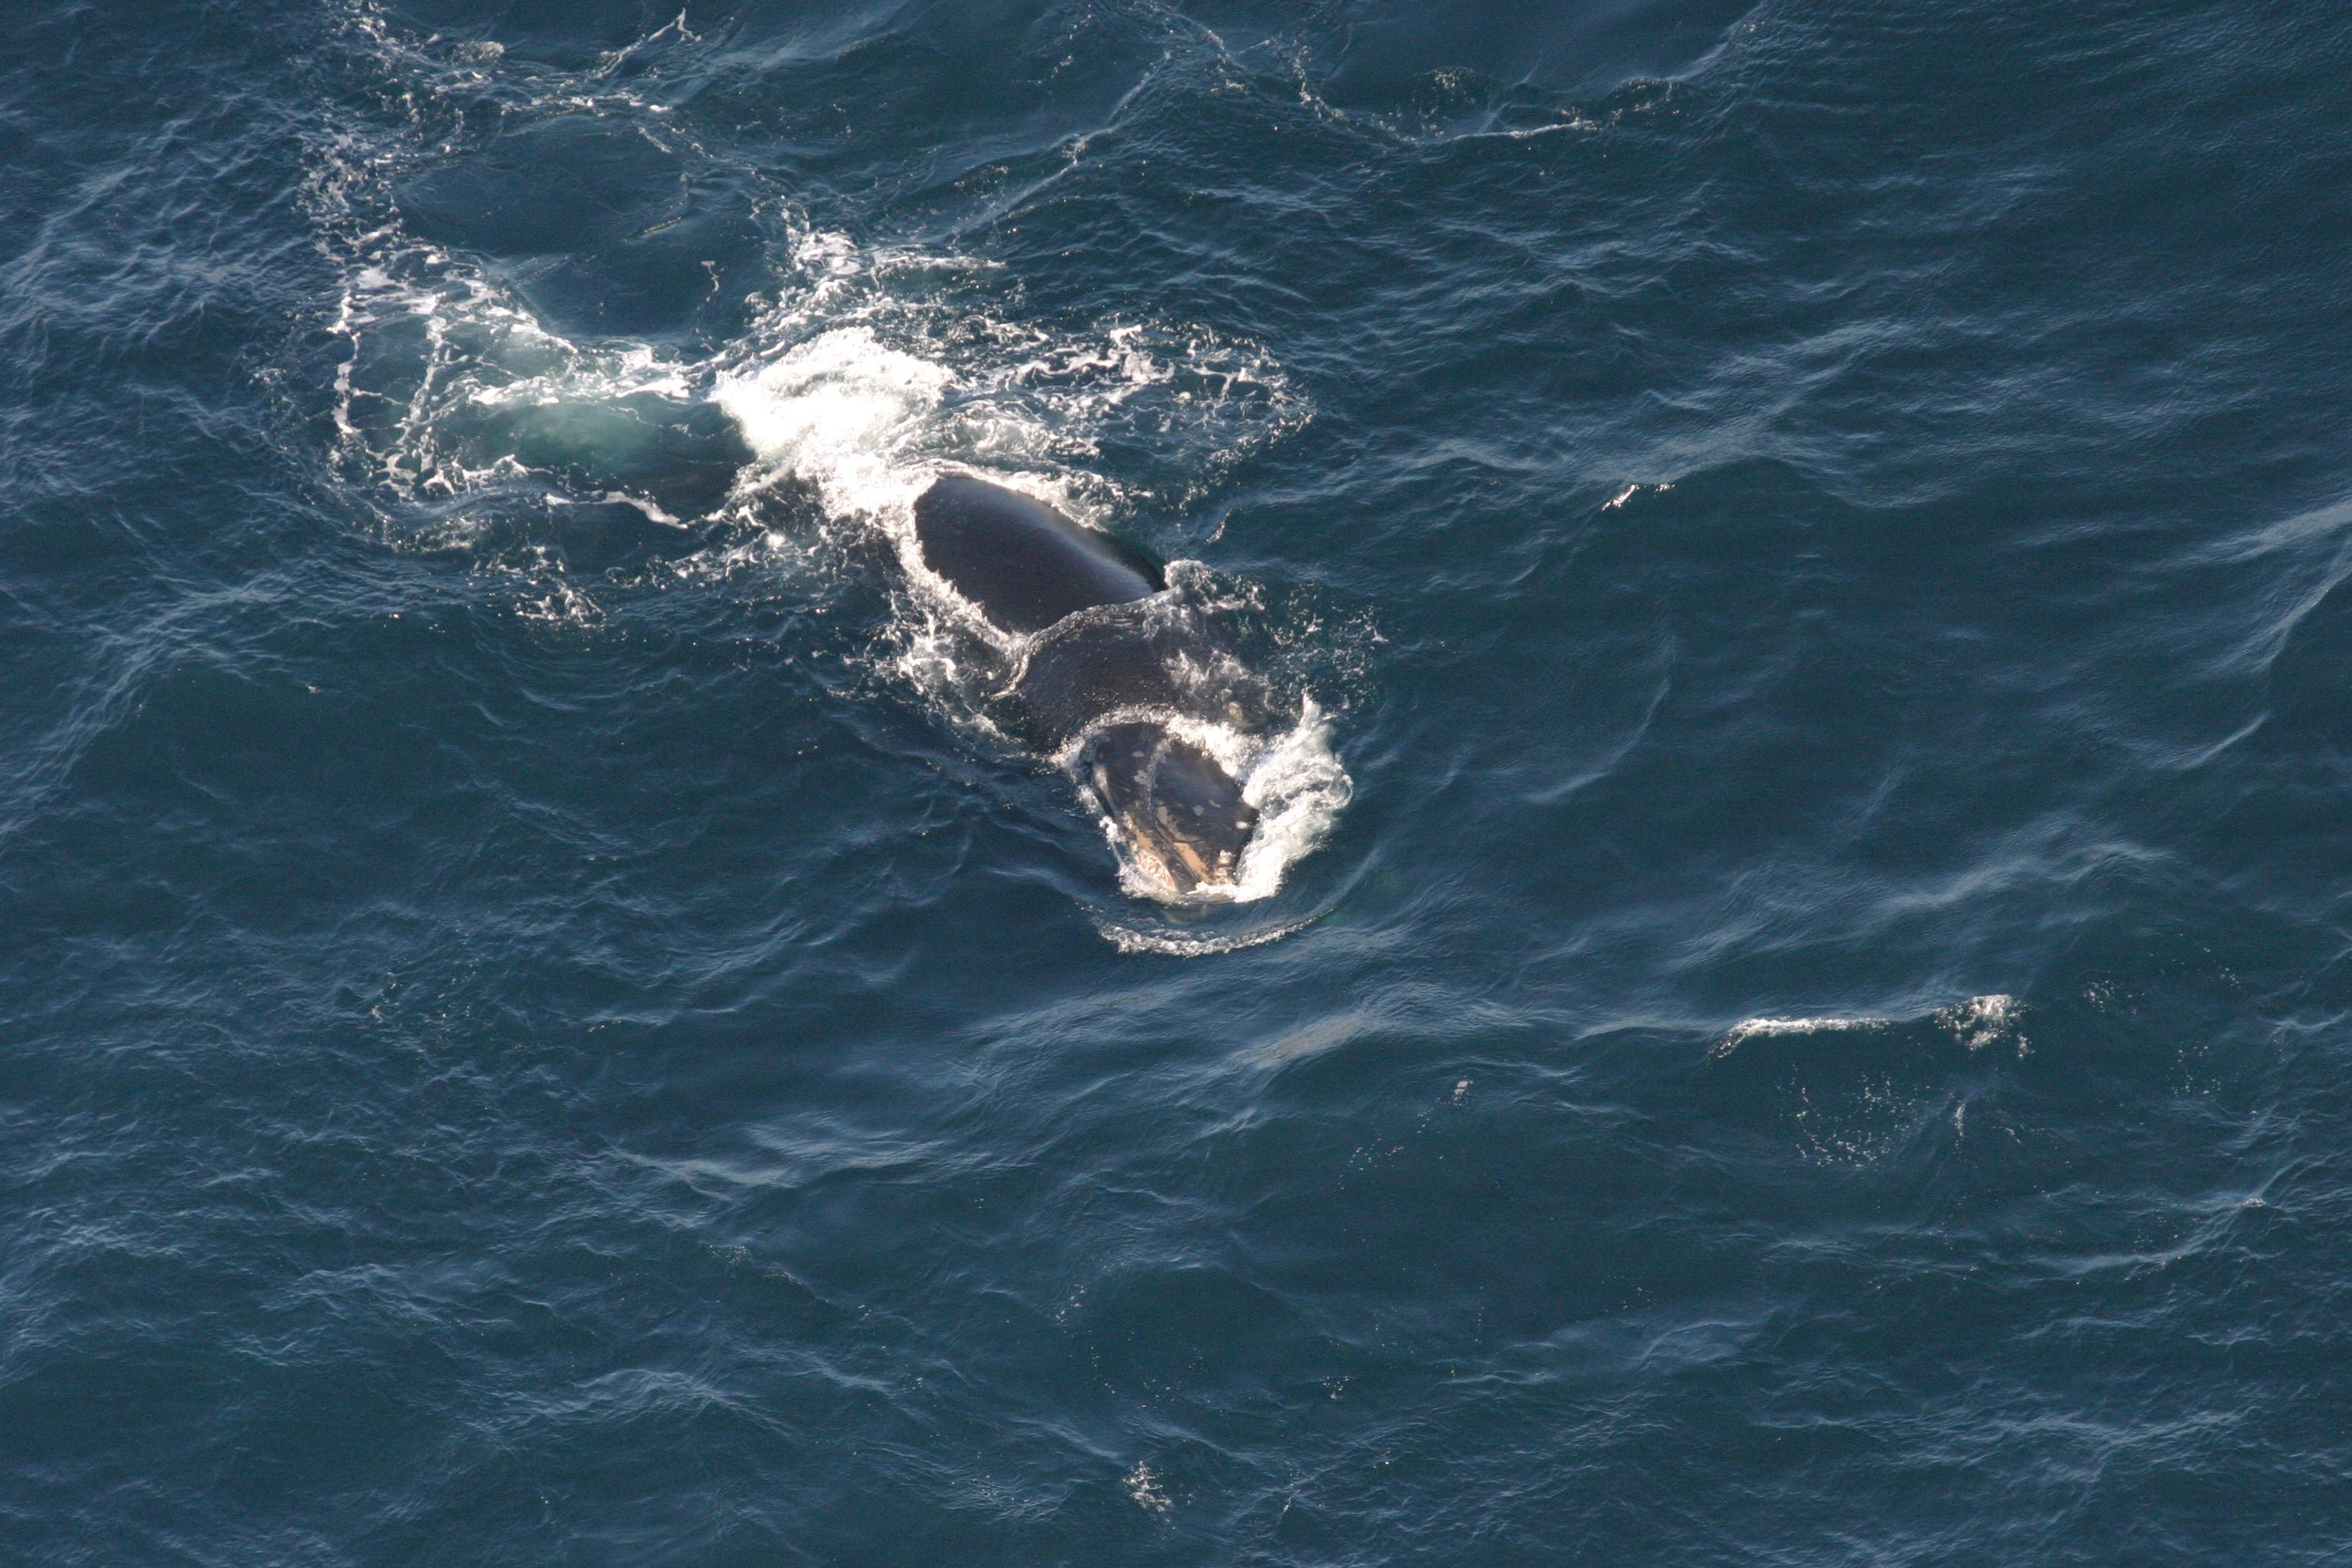
\includegraphics[scale=0.1]{foam.jpg}
	\caption{Example of a whale aerial picture with foam}
\end{figure}

\begin{figure}
	\centering
	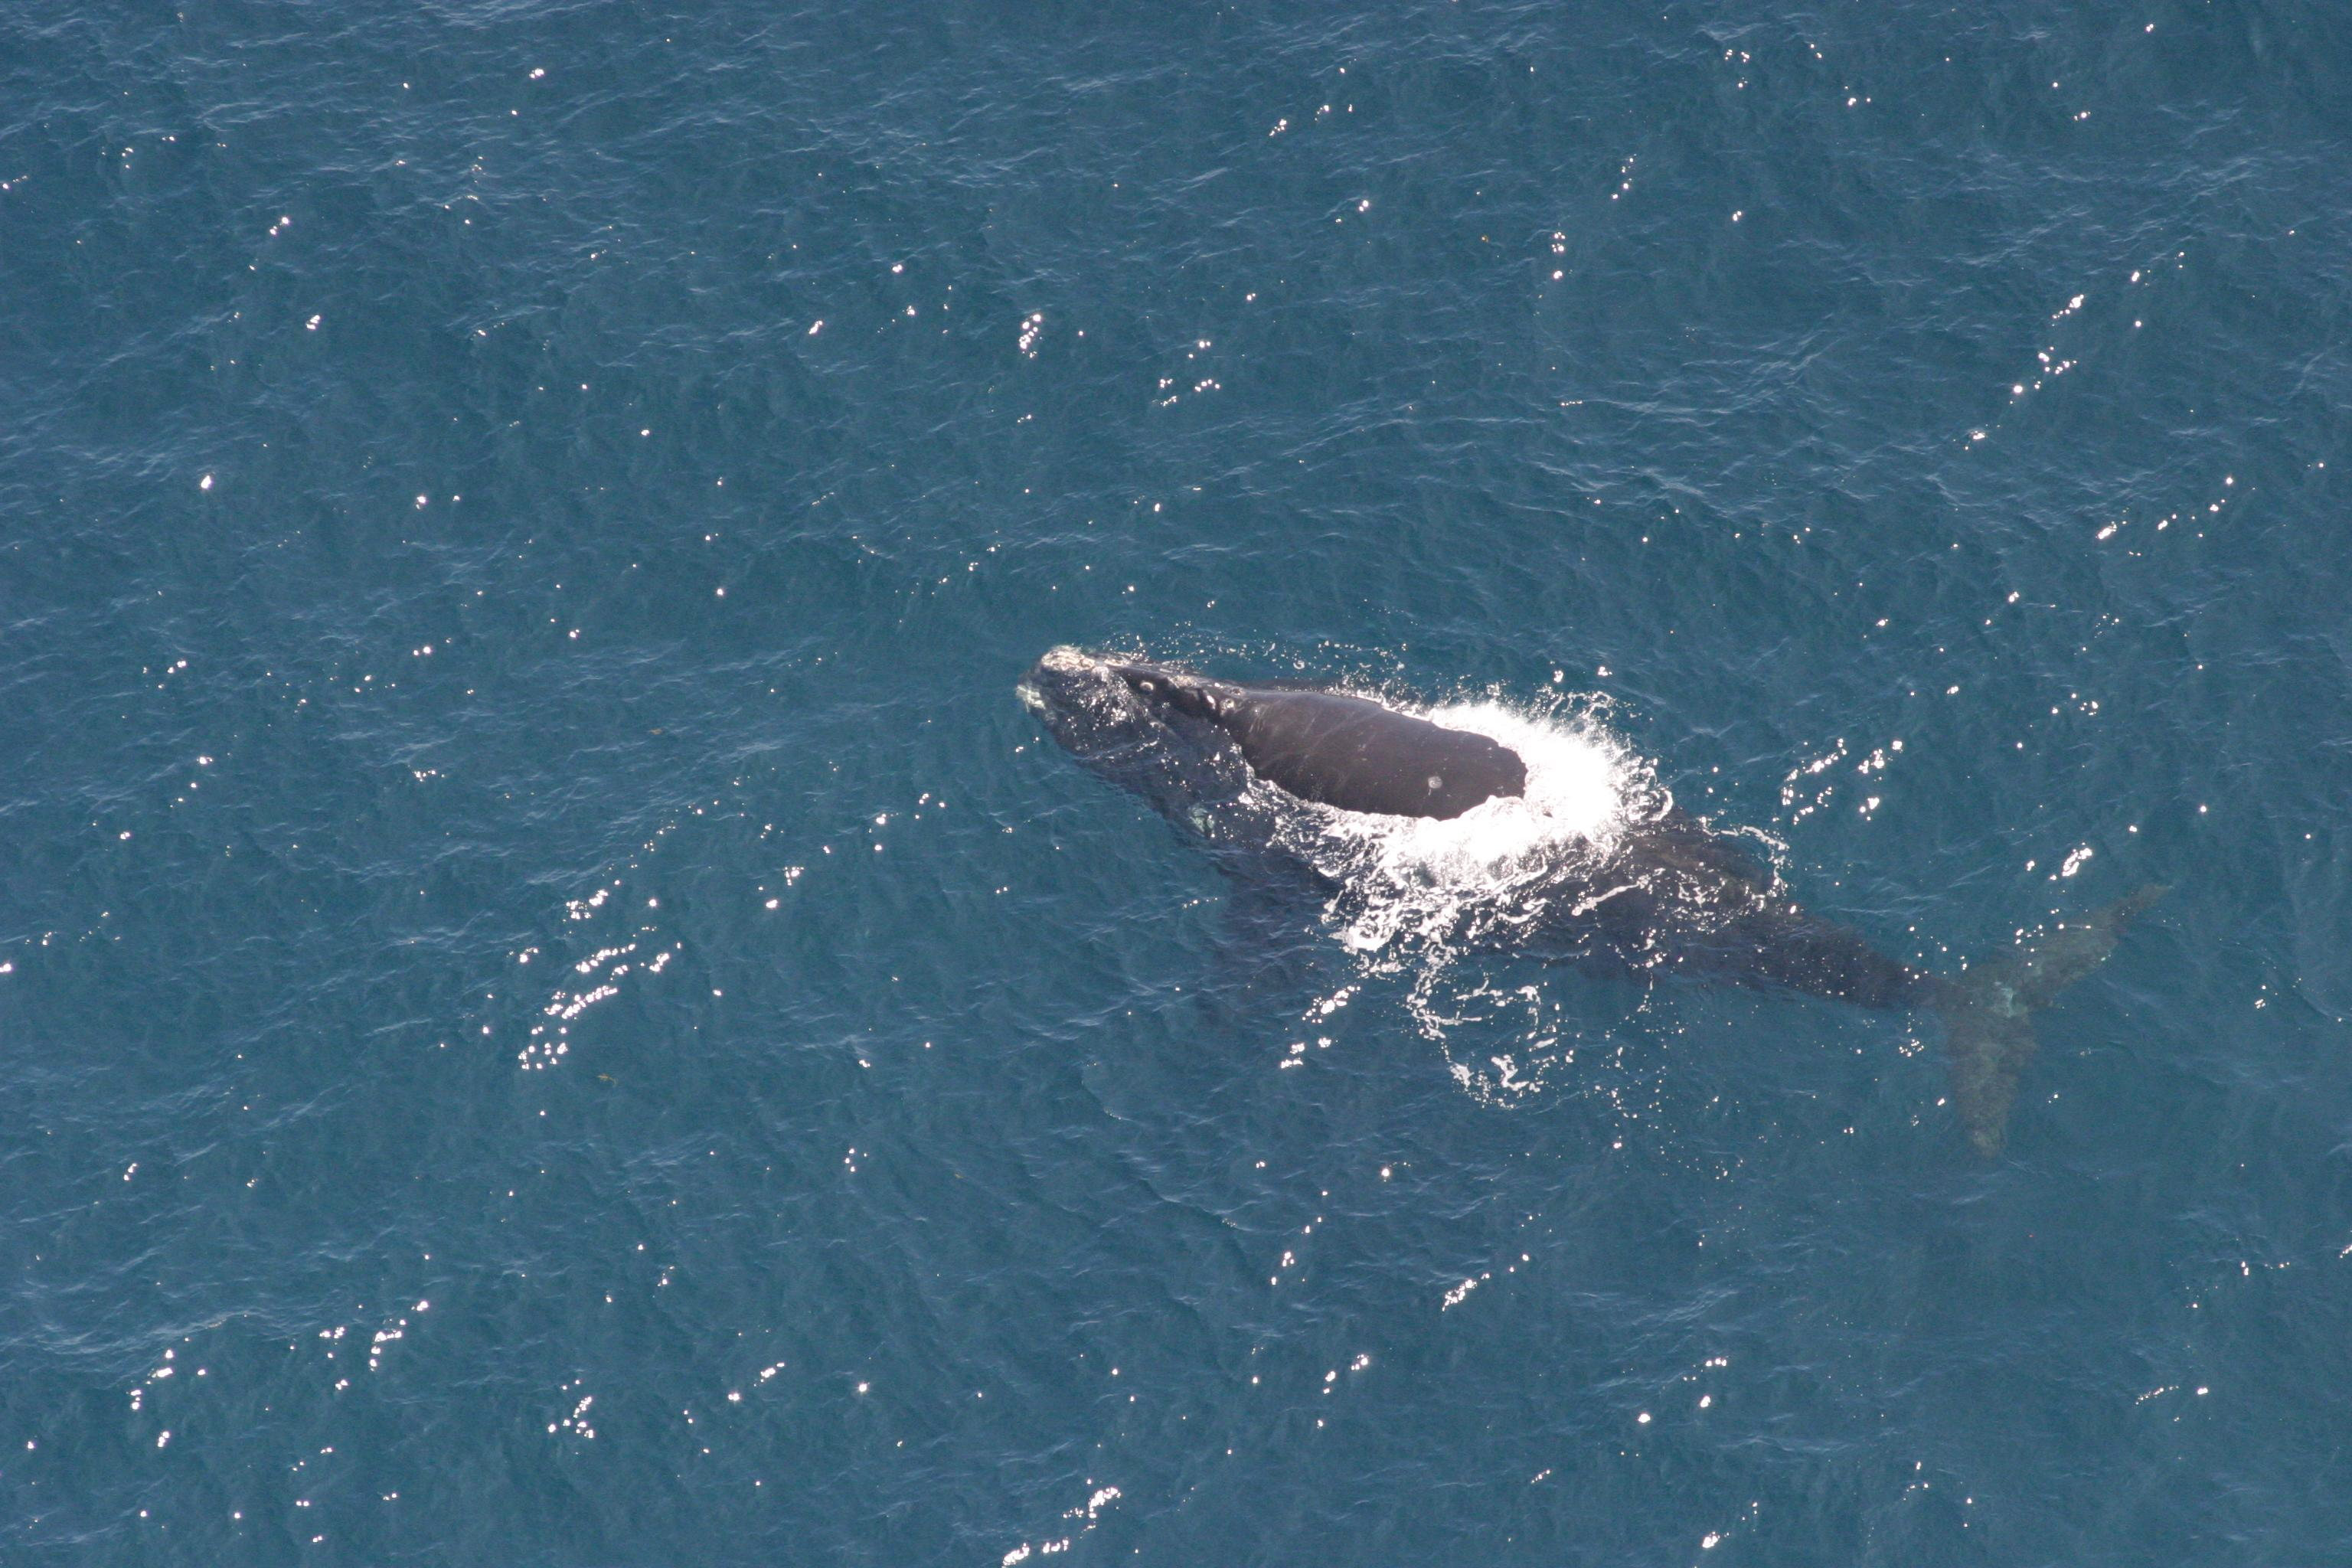
\includegraphics[scale=0.15]{water.jpg}
	\caption{Example of a whale aerial picture with shining water}
\end{figure}

\begin{figure}
	\centering
	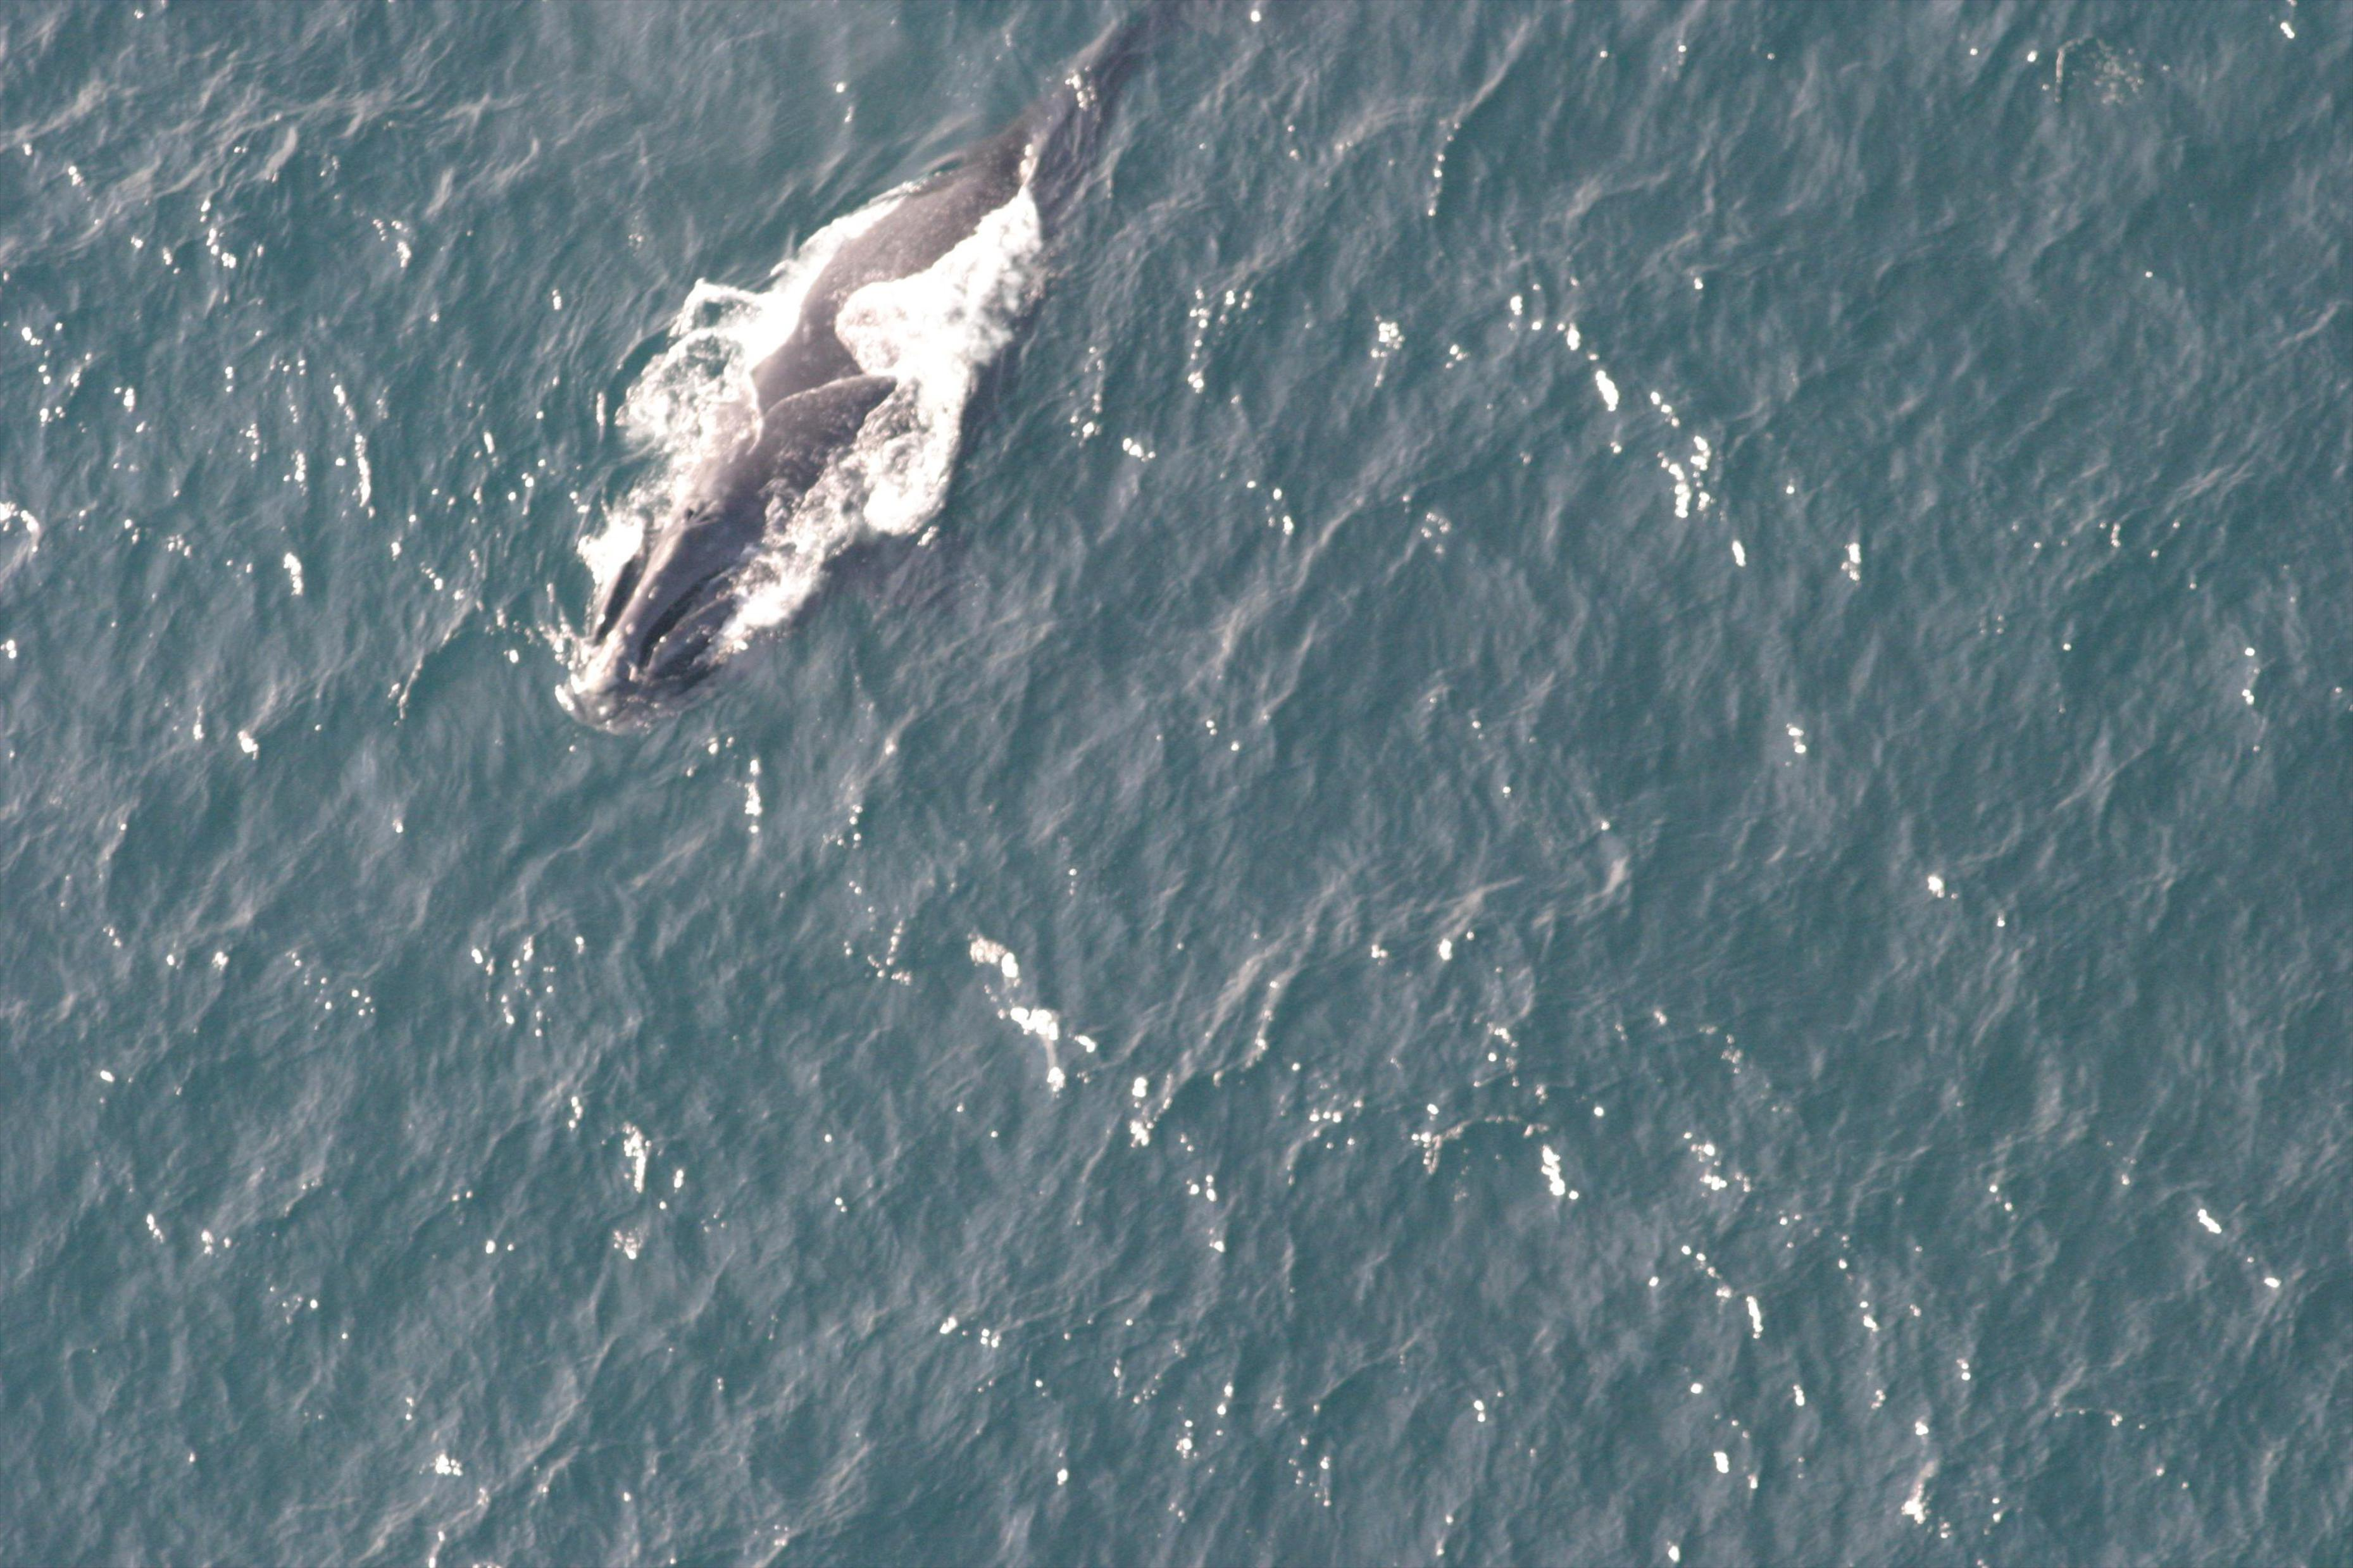
\includegraphics[scale=0.1]{invisible.jpg}
	\caption{Example of a whale aerial picture where the callosities are not visible}
\end{figure}

\begin{figure}
	\centering
	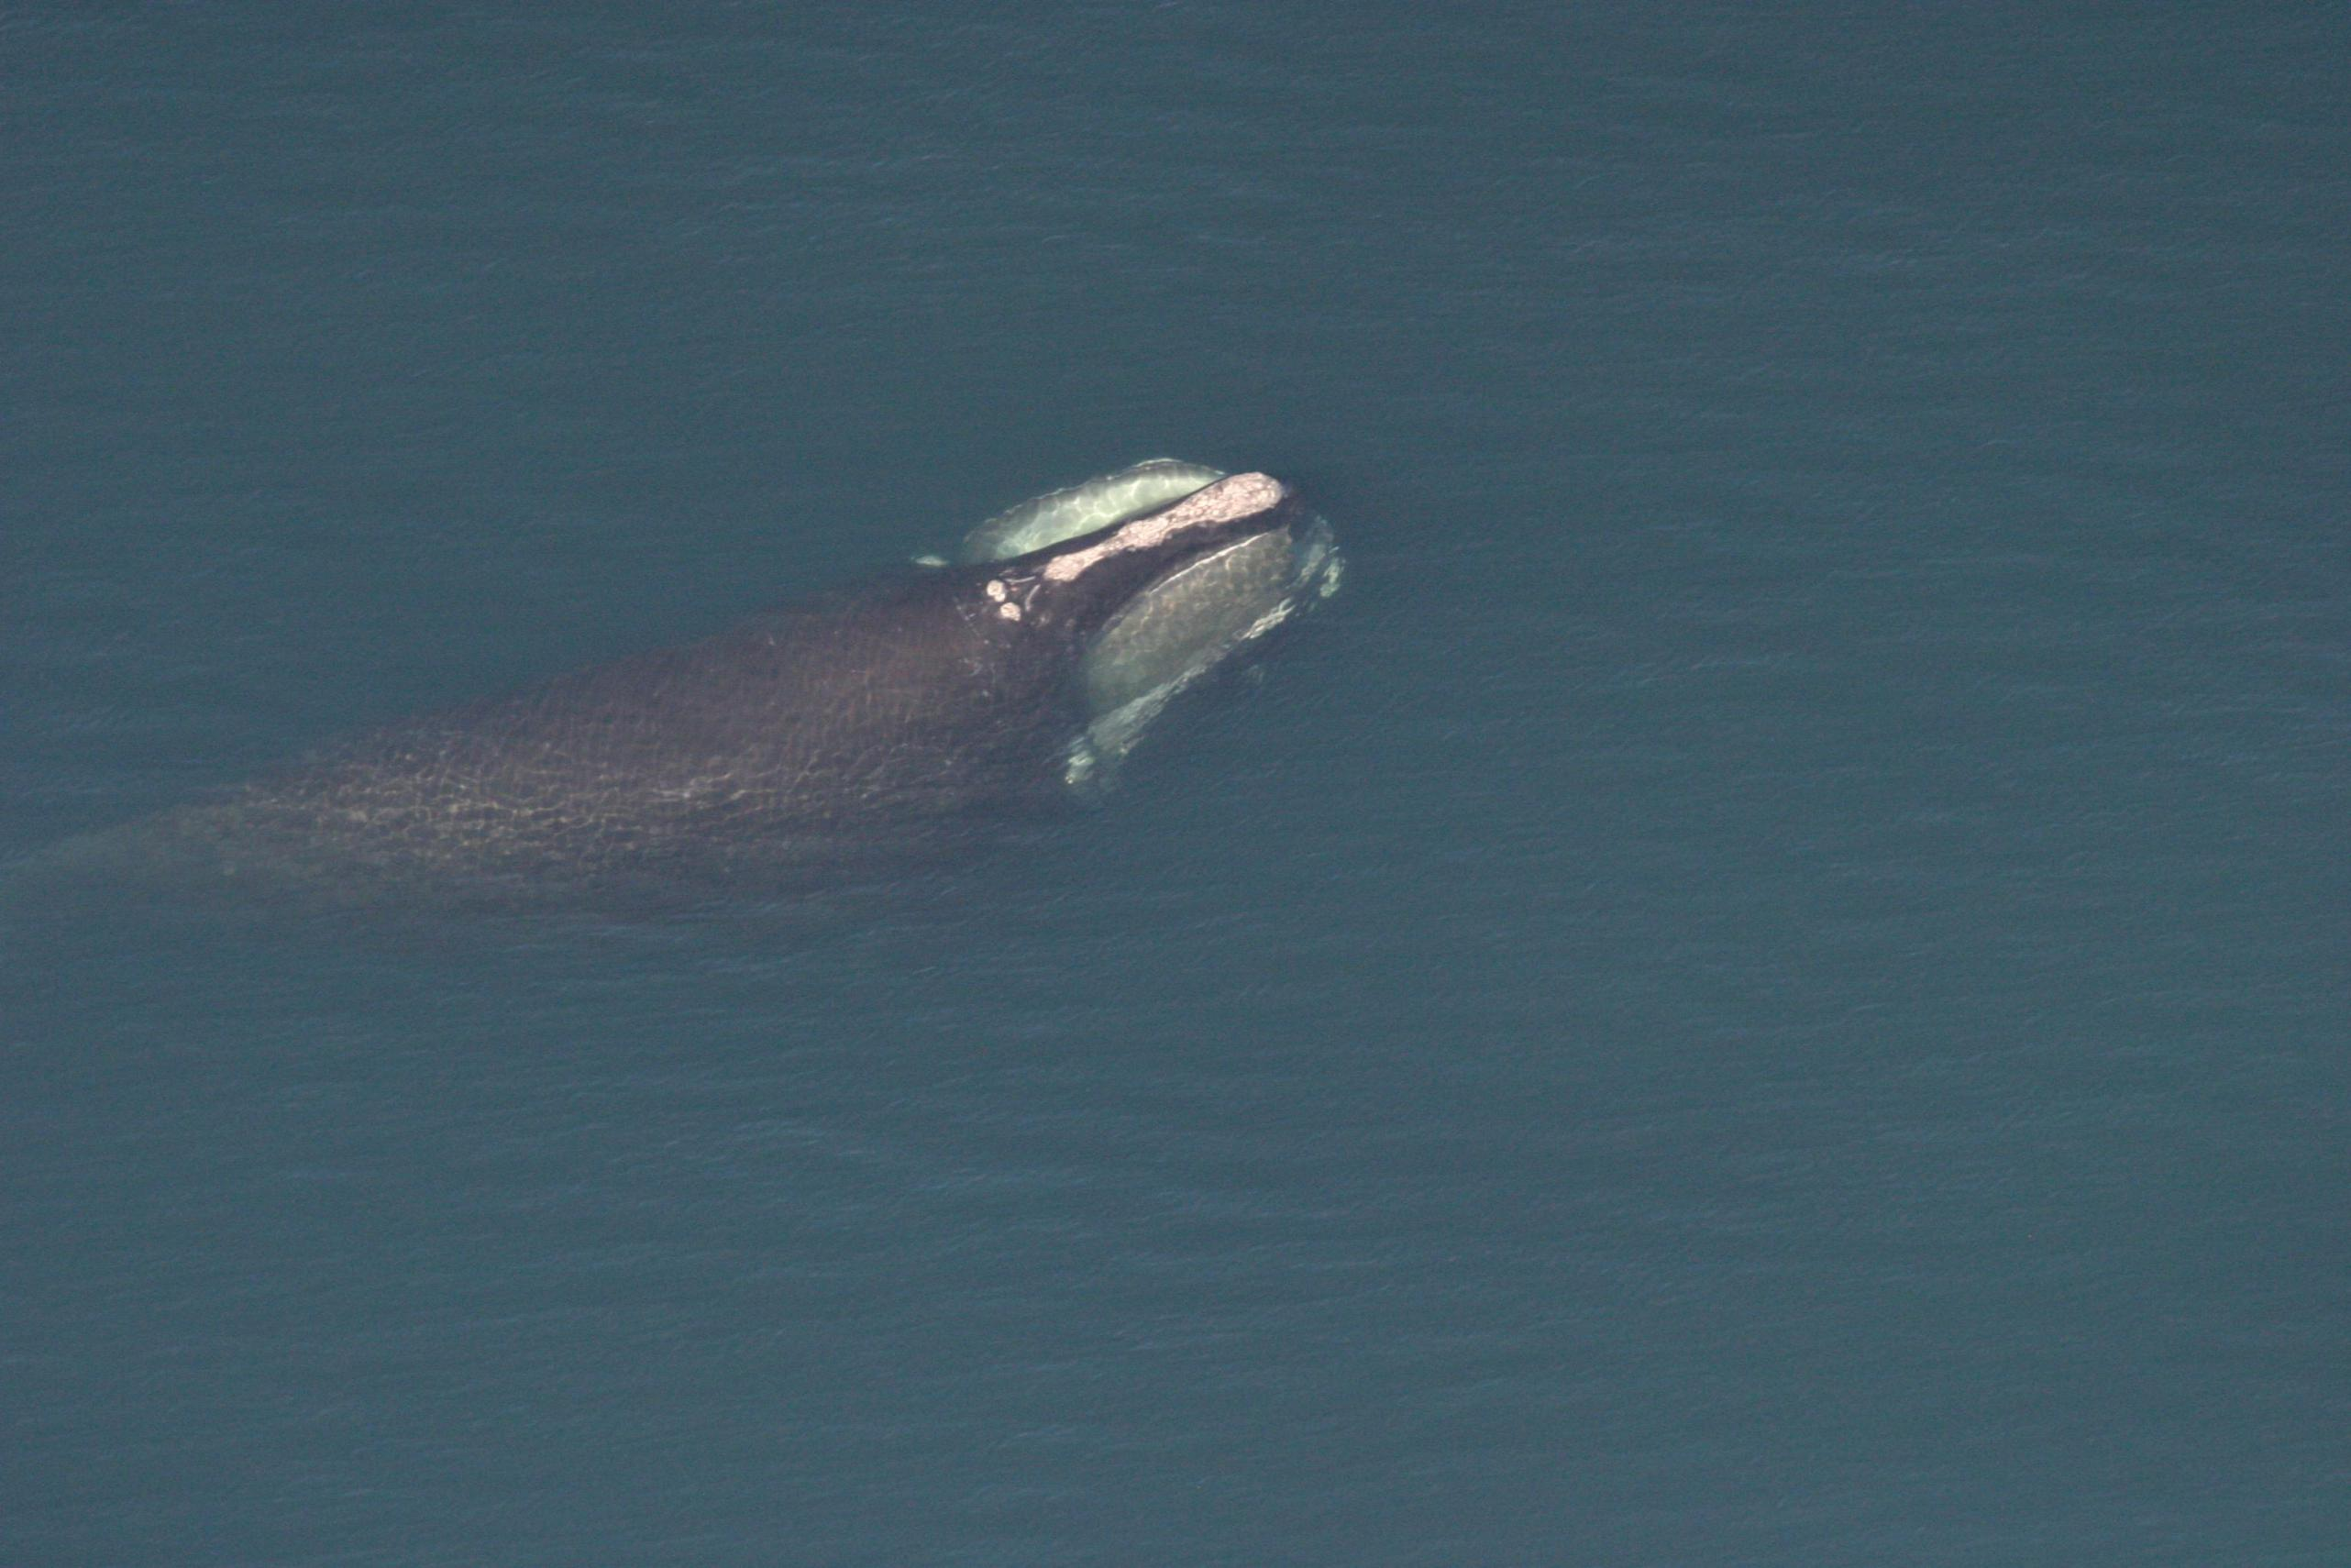
\includegraphics[scale=0.15]{better.jpg}
	\caption{Example of a relevant whale aerial picture}
\end{figure}

\end{appendices}

\bibliographystyle{unsrt}
\bibliography{bibliography.bib}

\end{document}
